\documentclass[aspectratio=169]{beamer}

% Quitar barra de navegación
\setbeamertemplate{navigation symbols}{}

% Paquetes para diseño y matemáticas
\usepackage{tikz}
\usetikzlibrary{positioning}
\usepackage[spanish]{babel}
\usepackage[utf8]{inputenc}
\usepackage{amsmath}
\usepackage{graphicx}
\graphicspath{{figures/}{./}}
\usepackage{hyperref}

% ------------------------------------------------------------------
%  Paleta de Colores (Estilo Dark Mode / Neon)
% ------------------------------------------------------------------
% Colores predeterminados (Fondo oscuro con acentos neon):
\definecolor{darkbg}{RGB}{24, 26, 27}       % Fondo principal oscuro
\definecolor{darkerbg}{RGB}{15, 16, 17}     % Fondo secundario para contrastes
\definecolor{neonblue}{RGB}{0, 195, 255}    % Azul brillante para acentos y títulos
\definecolor{lighttext}{RGB}{235, 235, 235} % Texto claro suave

% Alternativa: Paleta Light Mode (institucional / formal)
% \definecolor{darkbg}{RGB}{255, 255, 255}    % Blanco
% \definecolor{darkerbg}{RGB}{245, 245, 247}  % Gris tenue
% \definecolor{neonblue}{RGB}{0, 82, 155}     % Azul institucional
% \definecolor{lighttext}{RGB}{33, 37, 41}    % Texto oscuro

% Configuración global de Beamer para Dark Mode
\setbeamercolor{background canvas}{bg=darkbg}
\setbeamercolor{normal text}{fg=lighttext}
\setbeamercolor{math text}{fg=lighttext}
\setbeamercolor{frametitle}{fg=neonblue}
\setbeamerfont{frametitle}{series=\bfseries}
\setbeamertemplate{frametitle}{
    \vspace{0.4cm}
    \insertframetitle
    \par\color{neonblue}\rule{\textwidth}{0.5pt}
}

% Estilos de listas y bibliografía
\setbeamertemplate{itemize items}[circle]
\setbeamercolor{itemize item}{fg=neonblue}
\setbeamercolor{itemize subitem}{fg=neonblue}
\setbeamercolor{enumerate item}{fg=neonblue}
\setbeamercolor{item projected}{bg=neonblue, fg=darkbg}
\setbeamercolor{bibliography item}{fg=neonblue}
\setbeamercolor{bibliography entry author}{fg=lighttext}
\setbeamercolor{bibliography entry title}{fg=lighttext}
\setbeamercolor{bibliography entry location}{fg=lighttext}
\setbeamercolor{bibliography entry note}{fg=lighttext}

\begin{document}

% ---------------------------------------------------
% DIAPOSITIVA 1: PORTADA
% ---------------------------------------------------
\begin{frame}[plain]
\begin{tikzpicture}[remember picture, overlay]
    \fill[darkbg] (current page.south west) rectangle (current page.north east);
    \fill[darkerbg] (current page.south west) -- (current page.north east) -- (current page.south east) -- cycle;
    
    \node[anchor=west, text width=0.75\paperwidth, align=left] at ([xshift=0.8cm, yshift=1cm]current page.west) {
        \color{neonblue}\huge\textbf{Anillos de Newton}\\[0.4cm]
        \color{lighttext}\Large Interferencia en Películas Delgadas $\cdot$ Óptica Experimental
    };
    
    \node[anchor=south west, text width=0.8\paperwidth, align=left] at ([xshift=0.8cm, yshift=0.8cm]current page.south west) {
        \color{lighttext}\small \textbf{Autores:} Alan Ivan Ortega C., Luz Stefanía Pérez H., Ángel Gabriel Munguía V.\\
        Depto. de Actuaría, Física y Matemáticas, UDLAP\\
        \today
    };
\end{tikzpicture}
\end{frame}

% ---------------------------------------------------
% DIAPOSITIVA 2: OBJETIVOS
% ---------------------------------------------------
\begin{frame}{Objetivo y Metas Específicas}
    \textbf{\textcolor{neonblue}{Objetivo Principal}}
    \begin{itemize}
        \item Estudiar la interferencia en la película de aire formada entre una lente planoconvexa y una placa plana.
    \end{itemize}
    \vspace{0.4cm}
    \textbf{\textcolor{neonblue}{Metas Específicas}}
    \begin{enumerate}
        \item Observar y comparar los anillos de Newton en reflexión y transmisión.
        \item Relacionar su complementariedad con el cambio de fase por reflexión.
        \item Estimar la longitud de onda asociada a los bordes medidos mediante un ajuste lineal.
    \end{enumerate}
\end{frame}

% ---------------------------------------------------
% DIAPOSITIVA 3: MARCO TEÓRICO (PARTE 1)
% ---------------------------------------------------
\begin{frame}{Marco Teórico: Formación de los Anillos}
    \begin{columns}[T]
        \begin{column}{0.55\textwidth}
            \textbf{\textcolor{neonblue}{Película de aire}}
            \begin{itemize}
                \item Lente planoconvexa ($R = 12.144$ m) sobre placa plana.
                \item Se forma una cuña de aire de espesor variable $d$.
                \item Reflexión en dos interfaces: vidrio-aire y aire-vidrio.
                \item Cambio de fase de $\pi$ en la reflexión aire-vidrio.
            \end{itemize}
            \vspace{0.2cm}
            \textbf{\textcolor{neonblue}{Diferencia de camino óptico}}
            \begin{equation*}
                \Delta = 2d + \frac{\lambda}{2}
            \end{equation*}
        \end{column}
        \begin{column}{0.42\textwidth}
            \centering
            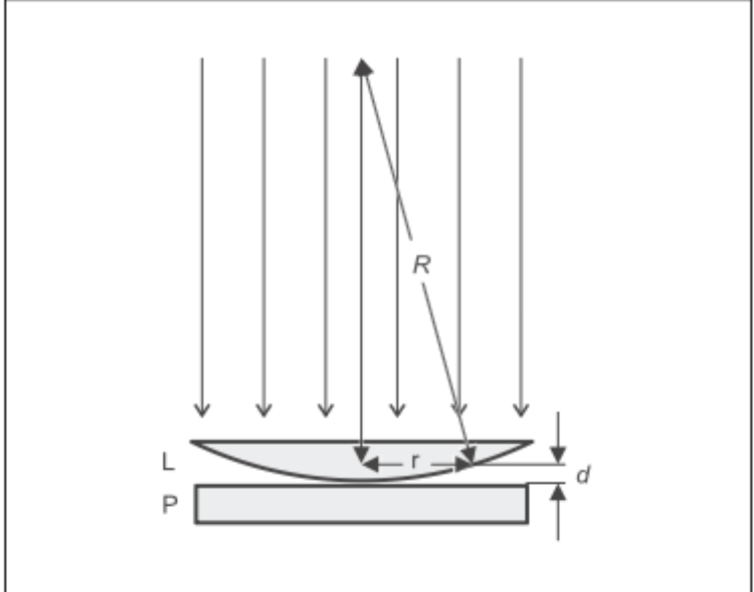
\includegraphics[width=\linewidth,height=7.5cm,keepaspectratio]{formacion_anillos.png}
        \end{column}
    \end{columns}
\end{frame}

% ---------------------------------------------------
% DIAPOSITIVA 4: MARCO TEÓRICO (PARTE 2)
% ---------------------------------------------------
\begin{frame}{Marco Teórico: Condiciones de Interferencia}
    \begin{columns}[c]
        \begin{column}{0.48\textwidth}
            \textbf{\textcolor{neonblue}{Espesor de la cuña}}
            \begin{equation*}
                d \approx \frac{r^2}{2R}
            \end{equation*}
            \vspace{0.2cm}
            \textbf{\textcolor{neonblue}{Anillos oscuros }}
            \begin{equation*}
                r_m = \sqrt{m \lambda R}
            \end{equation*}
            \textbf{\textcolor{neonblue}{Anillos brillantes }}
            \begin{equation*}
                r_m = \sqrt{\left(m + \tfrac{1}{2}\right) \lambda R}
            \end{equation*}
        \end{column}
        \begin{column}{0.48\textwidth}
            \centering
            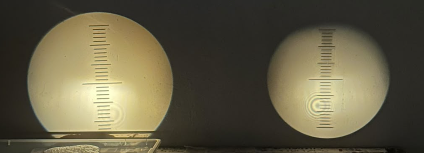
\includegraphics[width=\linewidth,height=5cm,keepaspectratio]{LAB 10 OP_Anillos Newton.png}
        \end{column}
    \end{columns}
\end{frame}

% ---------------------------------------------------
% DIAPOSITIVA 5: MAGNIFICACIÓN Y AJUSTE
% ---------------------------------------------------
% ---------------------------------------------------
% DIAPOSITIVA 6: MATERIALES Y MONTAJE
% ---------------------------------------------------
\begin{frame}{Materiales y Montaje Experimental}
    \begin{columns}[T]
        \begin{column}{0.45\textwidth}
            \textbf{\textcolor{neonblue}{Equipo}}
            \begin{itemize}
                \item 1. Lámpara de halógeno, 12 V
                \item Banco óptico
                \item 2 lentes $f=+200$ mm
                \item Transformador, 12 V
                \item 2 divisores de haz
                \item Placa de anillos de Newton
            \end{itemize}
        \end{column}
        \begin{column}{0.52\textwidth}
            \centering
            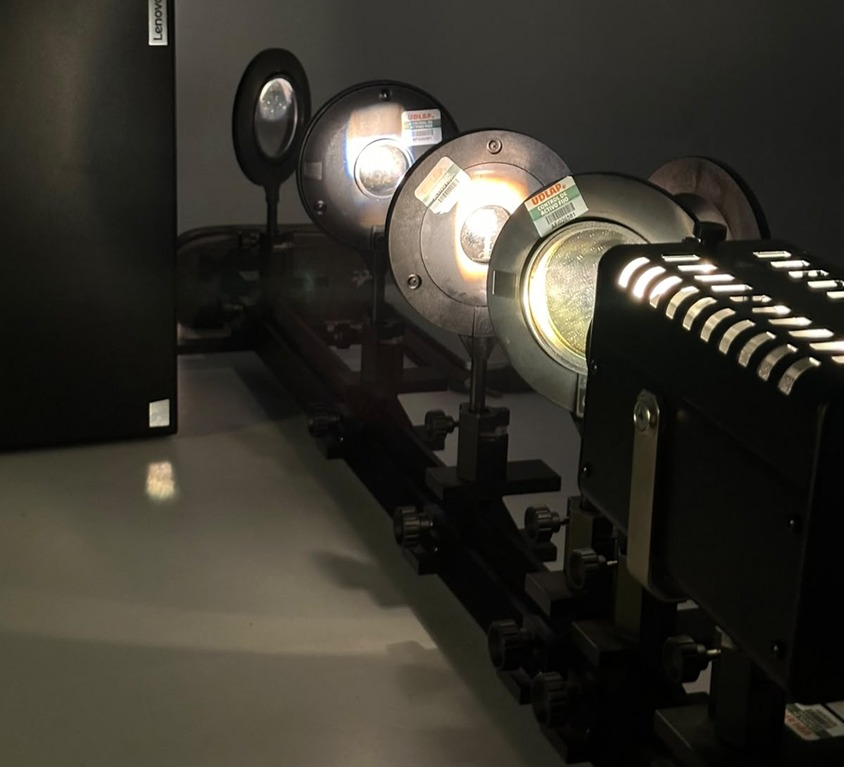
\includegraphics[width=\linewidth,height=4.5cm,keepaspectratio]{LAB 10 OP_Montaje.jpeg}
        \end{column}
    \end{columns}
\end{frame}

% ---------------------------------------------------
% DIAPOSITIVA 7: METODOLOGÍA — MONTAJE
% ---------------------------------------------------
\begin{frame}{Metodología: Montaje}
    \vfill
    \centering
    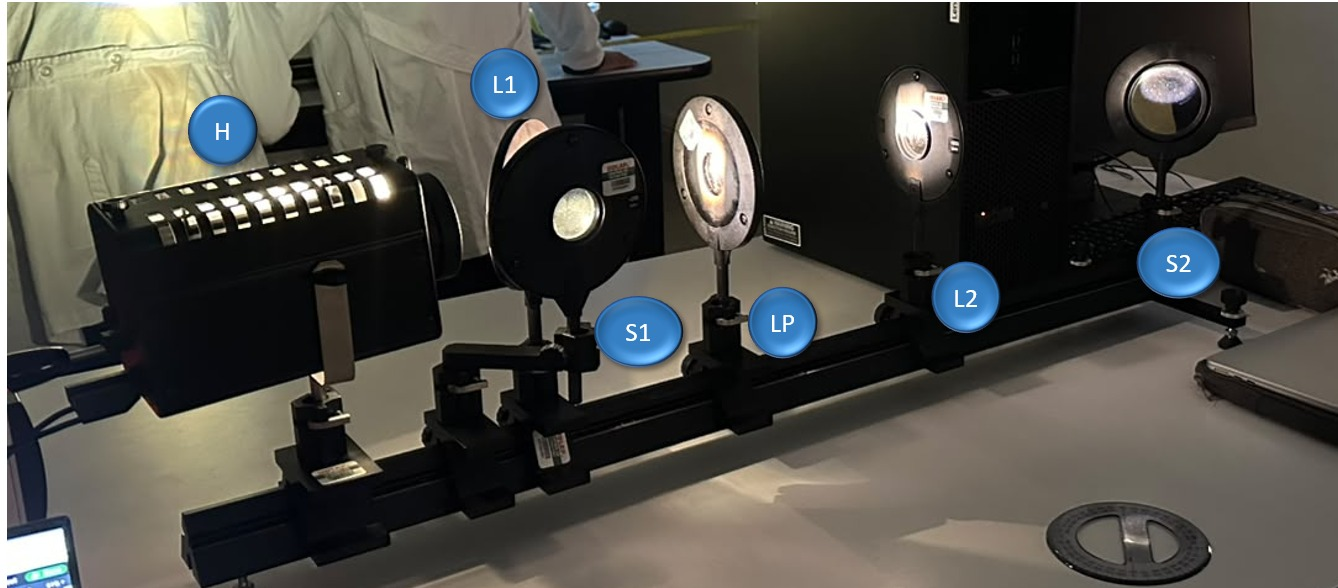
\includegraphics[width=0.85\textwidth,height=6cm,keepaspectratio]{arreglo_exp_met.jpeg}
    \vfill
\end{frame}

% ---------------------------------------------------
% DIAPOSITIVA 8: METODOLOGÍA — TOMA DE MEDICIONES
% ---------------------------------------------------
\begin{frame}[plain]
    \begin{tikzpicture}[remember picture, overlay]
        \node[inner sep=0] at (current page.center) {
            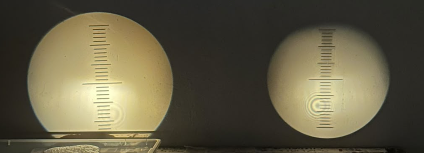
\includegraphics[width=\paperwidth,height=\paperheight]{LAB 10 OP_Anillos Newton.png}
        };
    \end{tikzpicture}
\end{frame}

% ---------------------------------------------------
% DIAPOSITIVA 9: DATOS EXPERIMENTALES
% ---------------------------------------------------
\begin{frame}{Datos Experimentales}
    \begin{columns}[T]
        \begin{column}{0.55\textwidth}
            \textbf{\textcolor{neonblue}{Diámetros proyectados ($\pm 0.005$ mm)}}
            \vspace{0.2cm}
            \begin{table}
                \centering
                \small
                \begin{tabular}{ccc}
                \hline
                \textbf{Anillo} & \textbf{Reflexión} & \textbf{Transmisión} \\ \hline
                Centro & 17.000 & 15.400 \\
                1 & 44.800 & 45.600 \\
                2 & 64.800 & 72.800 \\
                3 & 84.800 & 94.800 \\
                4 & 97.000 & 111.400 \\
                5 & 110.400 & 125.200 \\ \hline
                \end{tabular}
            \end{table}
        \end{column}
        \begin{column}{0.42\textwidth}
            \textbf{\textcolor{neonblue}{Distancias ($\pm 0.05$ cm)}}
            \vspace{0.2cm}
            \begin{table}
                \centering
                \small
                \begin{tabular}{ccc}
                \hline
                \textbf{Tray.} & \textbf{$g$} & \textbf{$b$} \\ \hline
                Reflexión & 22.09 & 210.51 \\
                Transmisión & 21.79 & 220.68 \\ \hline
                \end{tabular}
            \end{table}
            \vspace{0.3cm}
            \textbf{\textcolor{neonblue}{Magnificaciones}}
            \begin{itemize}
                \item $M_{\mathrm R} = 9.53 \pm 0.02$
                \item $M_{\mathrm T} = 10.13 \pm 0.02$
            \end{itemize}
        \end{column}
    \end{columns}
\end{frame}

% ---------------------------------------------------
% DIAPOSITIVA 10: AJUSTE EN REFLEXIÓN
% ---------------------------------------------------
\begin{frame}{Resultados: Ajuste en Reflexión}
    \begin{columns}[c]
        \begin{column}{0.55\textwidth}
            \centering
            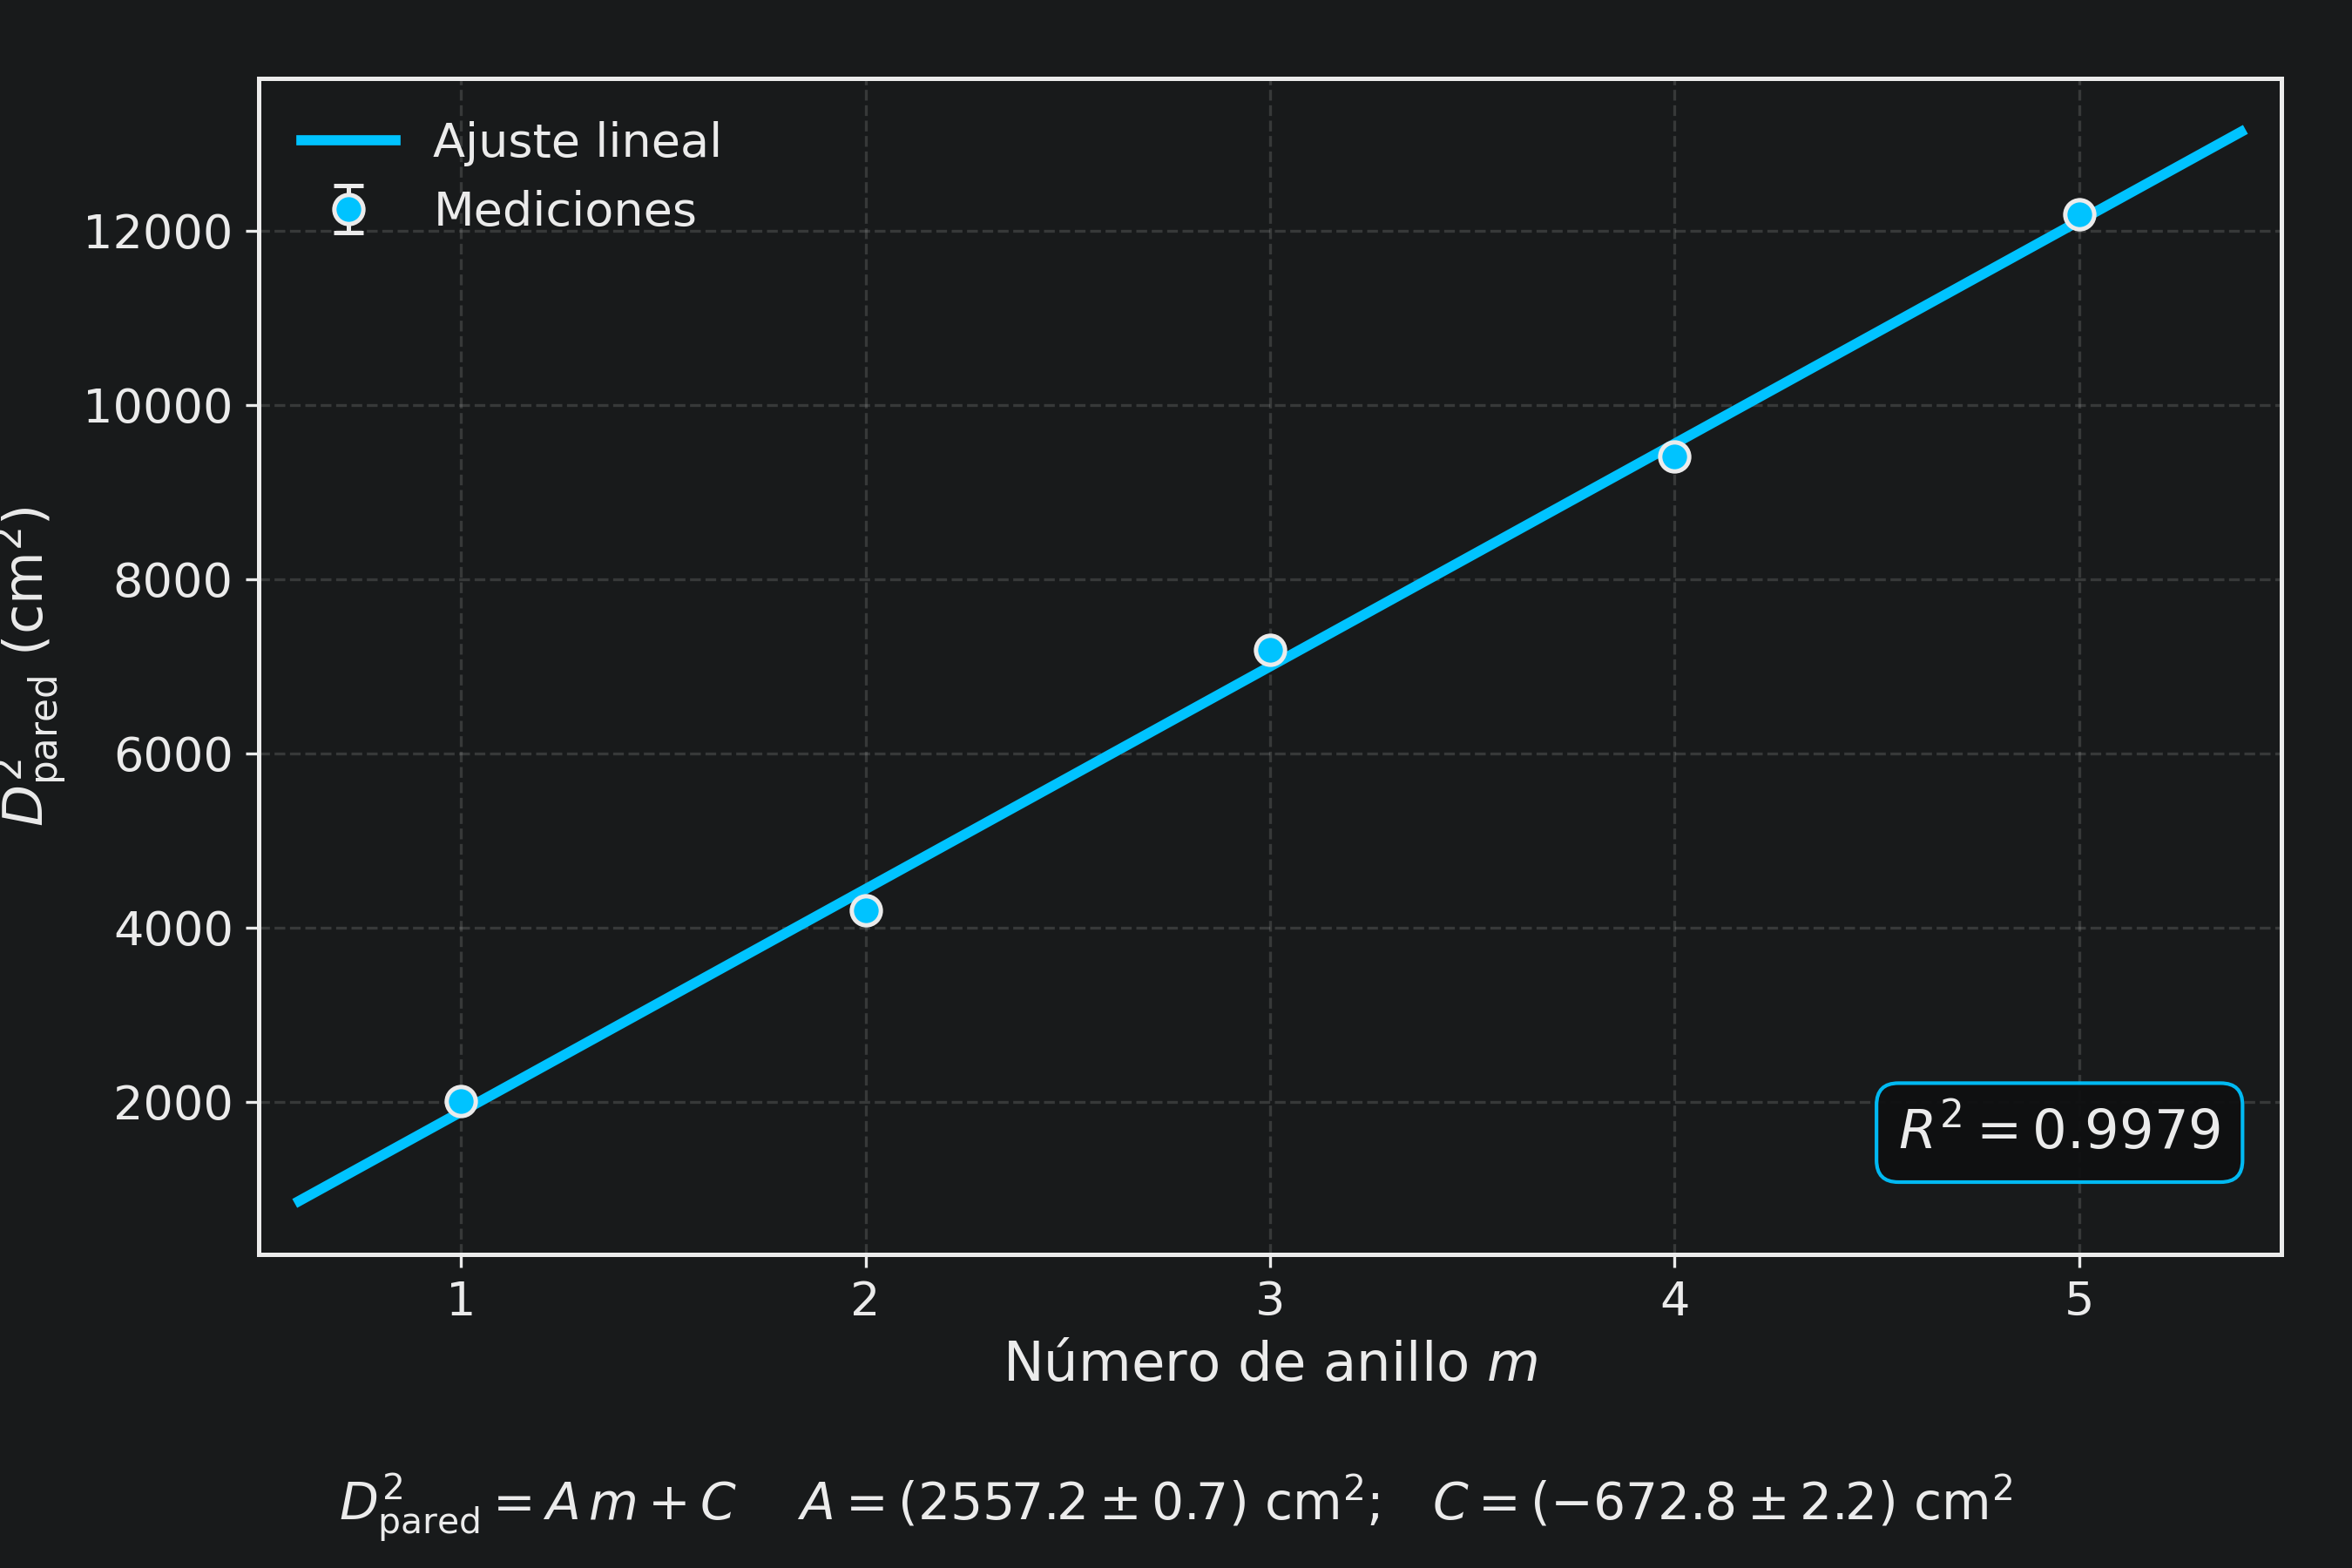
\includegraphics[width=\linewidth,height=5.5cm,keepaspectratio]{ajuste_reflexion.png}
        \end{column}
        \begin{column}{0.42\textwidth}
            \textbf{\textcolor{neonblue}{Parámetros del ajuste}}
            \begin{itemize}
                \item $A = (25.6 \pm 0.7)\ \mathrm{cm^2}$
                \item $C = (-6.7 \pm 2.2)\ \mathrm{cm^2}$
                \item $R^2 = 0.9979$
            \end{itemize}
            \vspace{0.3cm}
            \textbf{\textcolor{neonblue}{Longitud de onda}}
            \begin{equation*}
                \lambda_{\mathrm R} = (580 \pm 16)\ \mathrm{nm}
            \end{equation*}
        \end{column}
    \end{columns}
\end{frame}

% ---------------------------------------------------
% DIAPOSITIVA 11: AJUSTE EN TRANSMISIÓN
% ---------------------------------------------------
\begin{frame}{Resultados: Ajuste en Transmisión}
    \begin{columns}[c]
        \begin{column}{0.55\textwidth}
            \centering
            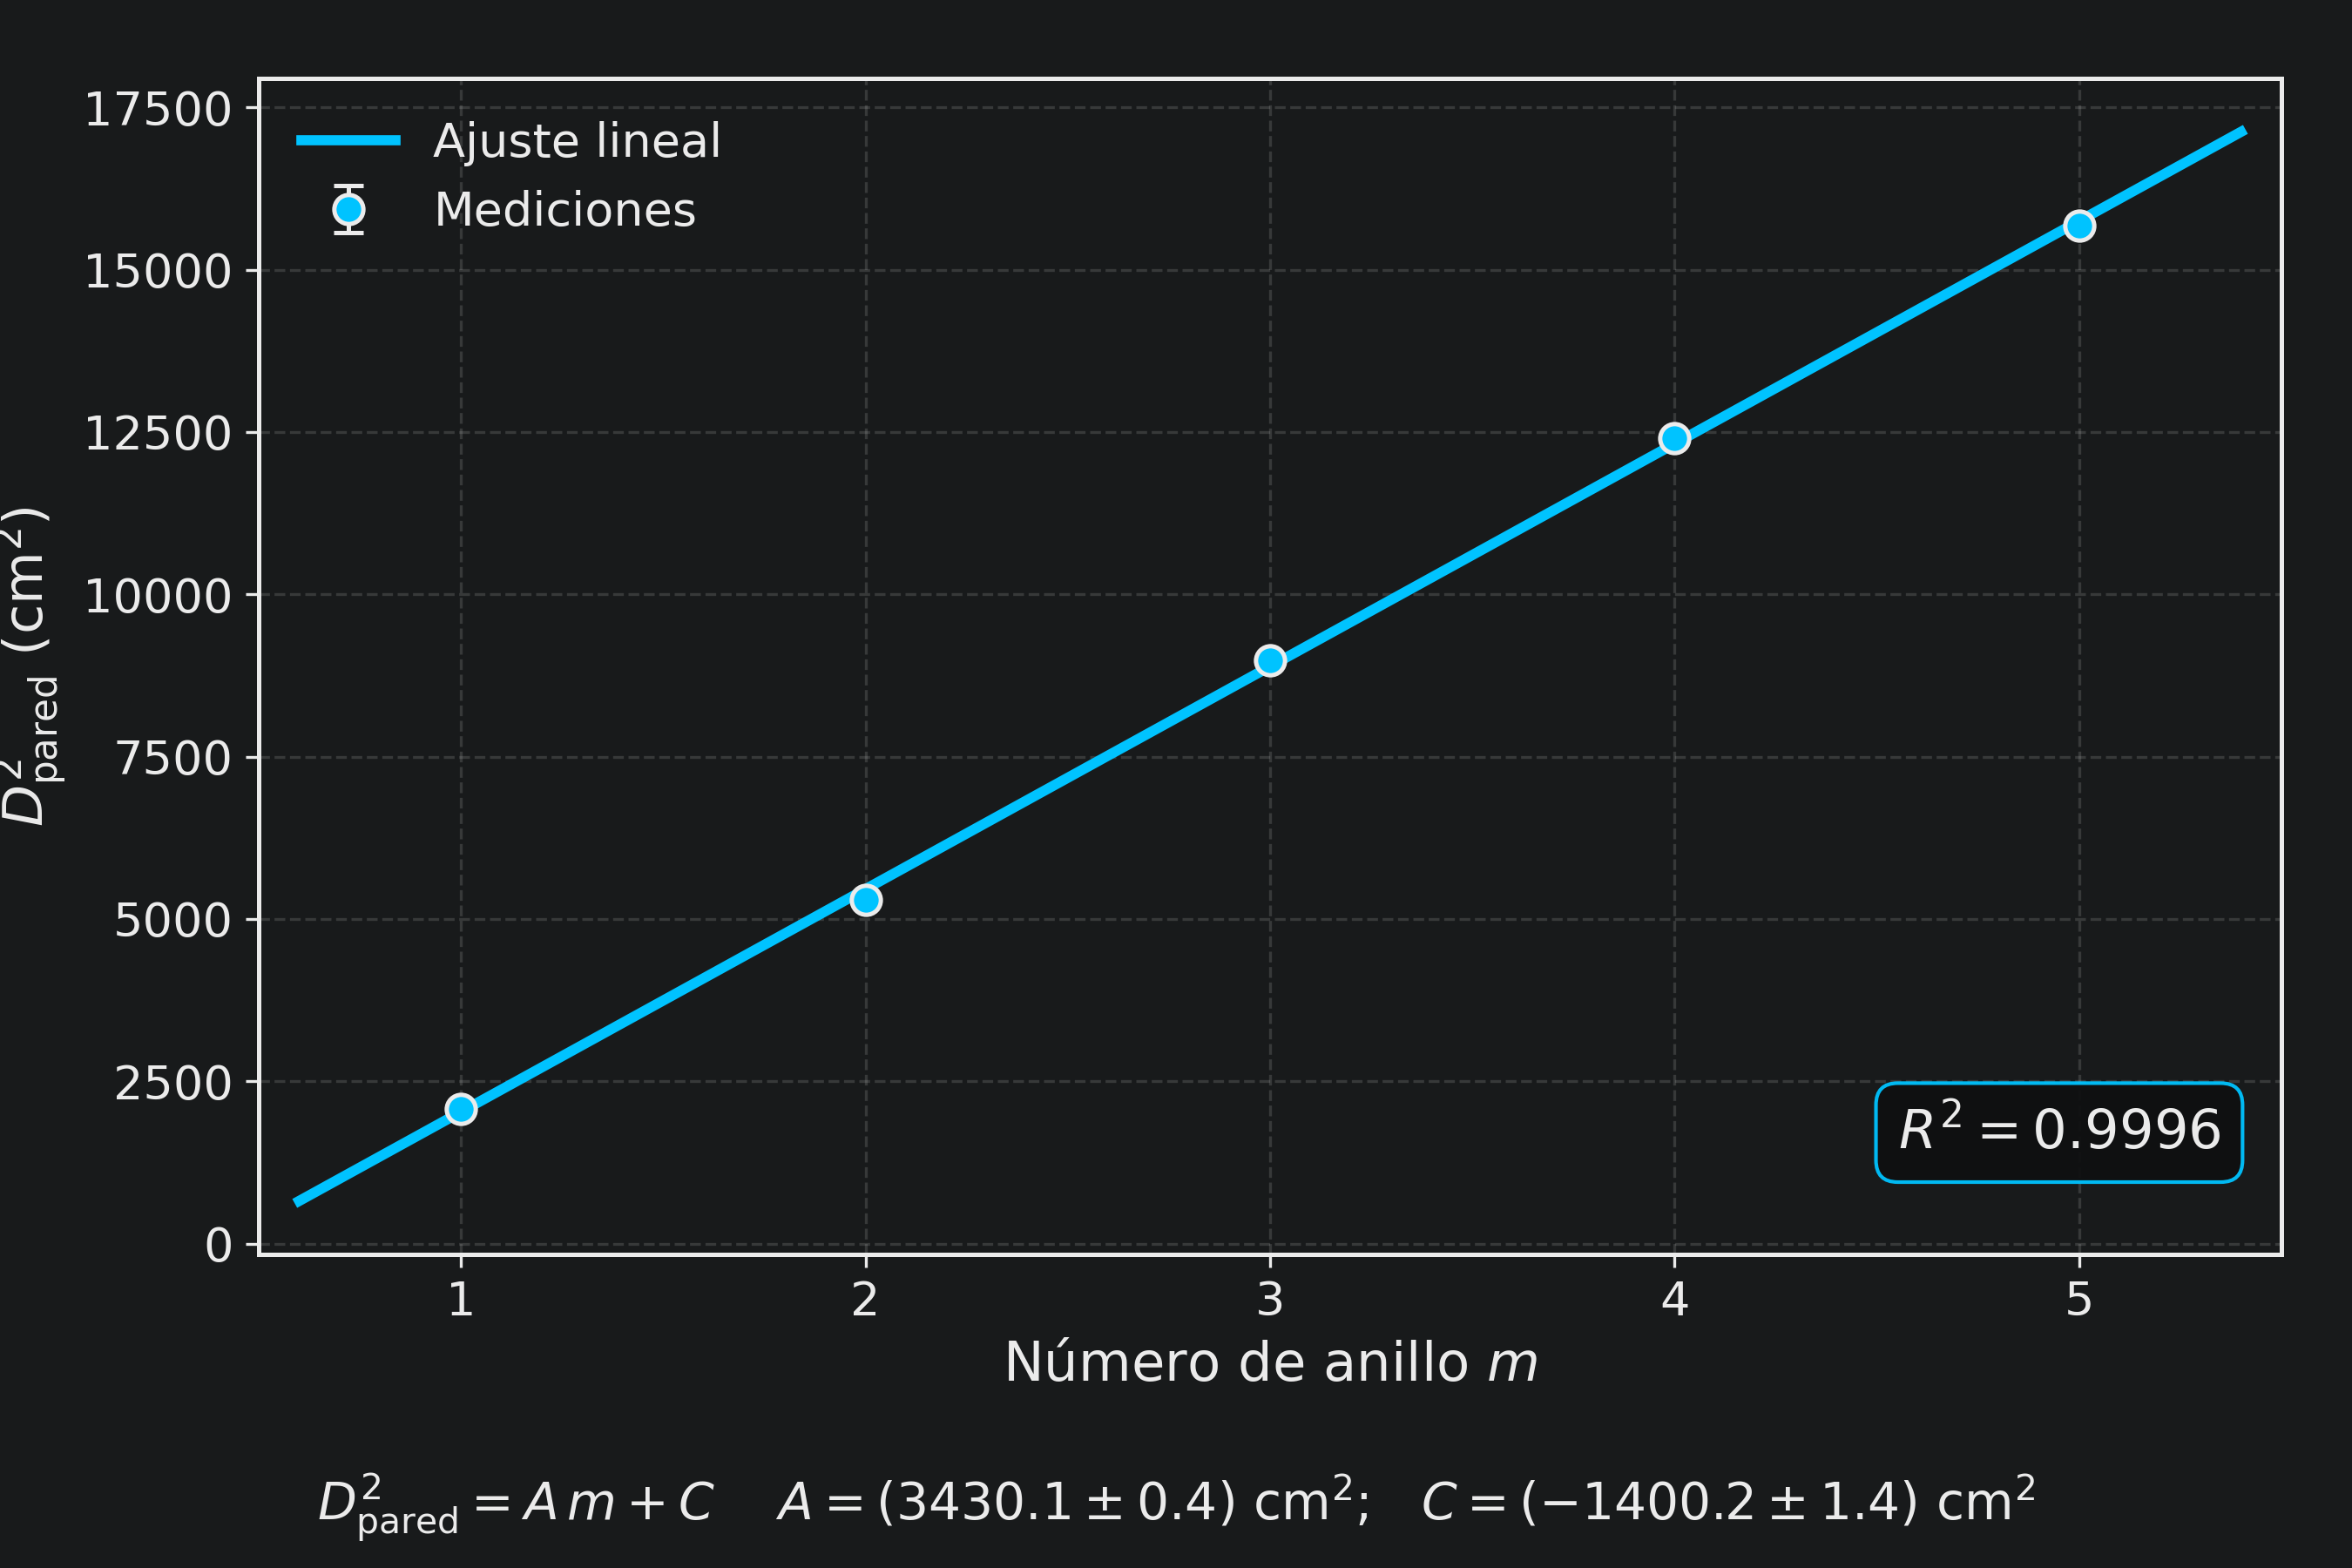
\includegraphics[width=\linewidth,height=5.5cm,keepaspectratio]{ajuste_transmision.png}
        \end{column}
        \begin{column}{0.42\textwidth}
            \textbf{\textcolor{neonblue}{Parámetros del ajuste}}
            \begin{itemize}
                \item $A = (34.3 \pm 0.4)\ \mathrm{cm^2}$
                \item $C = (-14.0 \pm 1.4)\ \mathrm{cm^2}$
                \item $R^2 = 0.9996$
            \end{itemize}
            \vspace{0.3cm}
            \textbf{\textcolor{neonblue}{Longitud de onda}}
            \begin{equation*}
                \lambda_{\mathrm T} = (688 \pm 9)\ \mathrm{nm}
            \end{equation*}
        \end{column}
    \end{columns}
\end{frame}

% ---------------------------------------------------
% DIAPOSITIVA 12: COMPARACIÓN Y ANÁLISIS
% ---------------------------------------------------
\begin{frame}{Comparación y Análisis}
    \begin{itemize}
        \item \textbf{\textcolor{neonblue}{Linealidad:}} Ambas series muestran dependencia aproximadamente lineal de $D_{\mathrm p}^2$ con $m$.
        \vspace{0.2cm}
        \item \textbf{\textcolor{neonblue}{Discrepancia entre $\lambda$:}} $(580 \pm 16)$ nm vs. $(688 \pm 9)$ nm. No coinciden dentro de incertidumbres.
        \vspace{0.2cm}
        \item \textbf{\textcolor{neonblue}{Posibles causas:}}
        \begin{itemize}
            \item Selección del borde en luz blanca (distintos colores).
            \item Calibración de la proyección.
            \item Diferencia de magnificación entre trayectorias (ya incluida).
        \end{itemize}
        \vspace{0.2cm}
        \item \textbf{\textcolor{neonblue}{Nota:}} Los 650 nm del manual corresponden a un ejemplo con bordes rojizos, no a un valor de referencia único.
    \end{itemize}
\end{frame}

% ---------------------------------------------------
% DIAPOSITIVA 13: CONCLUSIONES
% ---------------------------------------------------
\begin{frame}{Conclusiones}
    Se estudió la formación de anillos de Newton en reflexión y transmisión:
    \vspace{0.3cm}
    \begin{enumerate}
        \item \textbf{\textcolor{neonblue}{Reflexión:}} $\lambda_{\mathrm R} = (580 \pm 16)$ nm, con $R^2 = 0.9979$.
        \vspace{0.2cm}
        \item \textbf{\textcolor{neonblue}{Transmisión:}} $\lambda_{\mathrm T} = (688 \pm 9)$ nm, con $R^2 = 0.9996$.
        \vspace{0.2cm}
        \item \textbf{\textcolor{neonblue}{Linealidad:}} La dependencia de $D_{\mathrm p}^2$ con $m$ fue aproximadamente lineal en ambas series.
        \vspace{0.2cm}
        \item \textbf{\textcolor{neonblue}{Discrepancia:}} Las longitudes de onda no coinciden dentro de las incertidumbres; se atribuye a la selección de bordes en luz blanca y a la calibración de la proyección.
    \end{enumerate}
\end{frame}

% ---------------------------------------------------
% DIAPOSITIVA 14: REFERENCIAS
% ---------------------------------------------------
\begin{frame}{Referencias Bibliográficas}
    \begin{thebibliography}{9}
        \bibitem{LD_Physics} 
        LD DIDACTIC GmbH. 
        \textit{Newton's rings in transmitted and reflected white light}. 
        Physics Leaflets P5.3.3.2, pp.~1--4, 0713-Bi.
        
        \bibitem{Taylor} 
        Taylor, J. R. (1997). 
        \textit{An Introduction to Error Analysis} (2nd ed.). University Science Books.
        
        \bibitem{Hughes} 
        Hughes, I., \& Hase, T. (2010). 
        \textit{Measurements and Their Uncertainties: A Practical Guide to Modern Error Analysis}. Oxford University Press.
    \end{thebibliography}
\end{frame}

% ---------------------------------------------------
% DIAPOSITIVA 15: CIERRE
% ---------------------------------------------------
\begin{frame}[plain]
\begin{tikzpicture}[remember picture, overlay]
    \fill[darkbg] (current page.south west) rectangle (current page.north east);
    \fill[darkerbg] (current page.north west) -- (current page.south west) -- (current page.south east) -- cycle;
    
    \node[text=lighttext, font=\Huge\bfseries, align=center] at (current page.center) {
        ¡Gracias por su atención!\\[0.5cm]
    };
\end{tikzpicture}
\end{frame}

\end{document}